\chapter{Finite-size Effects}

In this chapter, I will describe the common types of finite size effects encountered in electronic structure simulations and a few correction schemes. I will begin the discussion from the most general correction that works for quantum and classical systems at zero or finite temperature: the static structure factor correction to the potential energy. From there, the method is extended to correct kinetic energy from the momentum distribution, and in the quantum case, the Jastrow pair function. %Then, I will discuss the dominant single-particle kinetic finite size effect in fermion systems, the so-called "shell filling" effects.
%Many-body corrections beyond pair interactions are outside the scope of this discussion.

\section{Correction to the potential energy}

\subsection{General Theory}
Given a simulation using periodic boundary conditions, the accessible momenta are quantized. As the simulation cell is enlarged, the grid of accessible momenta becomes finer until it grants access to the full continuum of momentum space in the thermodynamic limit. By considering the difference between this infinite system and the finite simulation cell, we can understand finite-size effects and attempt to correct them.
Consider an orthorhombic box with side length $L_x$ along the x direction. The momentum along the $x$ direction must take discrete values $k_x=\dfrac{2\pi}{L_x}n_x$, where $n_x\in\mathcal{N}$. Similarly discretization exist along the other directions.
%For simulations with the Coulomb interaction, one has no access to the $\bs{k}=\bs{0}$ volume element in reciprocal space.
In a simulation where particles interact via the Coulomb pair potential $v(r)=\frac{1}{r}$, the total potential energy of the system %can be written as an integral over the pair correlation function
\begin{align}
V \equiv V_{\text{background}} +
\frac{1}{2}\sum\limits_{i=1}^N
\sum\limits_{\bs{L}}\sum\limits_{j=1}^N
v(\vert\bs{x}_i-\bs{x}_j-\bs{L}\vert),
%= \frac{1}{\Omega}\int d\bs{x} g(\bs{x}) v(\bs{x}),
\end{align}
where $\bs{L}$ loop over the supercell lattice.
The sums loop over all pairs of particles in the infinite system.
%\begin{align}
%g(\bs{r}) \equiv \sum\limits_{i=1}^N\sum\limits_{j>i}^N \delta(\bs{r}-(\bs{r}_i-\bs{r}_j)).
%\end{align}
This equation can be equivalently written in reciprocal space as
\begin{align} \label{eq:fsc-vn-vk}
V_N \equiv V/N = v_M + \frac{1}{2\Omega} \sum\limits_{\bs{k}\neq\bs{0}} v_{\bs{k}} S(\bs{k}),
\end{align}
where $v_{\bs{k}}=\dfrac{2\pi (d-1)}{k^{d-1}}$ is the Fourier transform of the Coulomb pair potential in $d$ spatial dimensions. $v_M$ is the Madelung constant, which combines the electrostatic energy of an infinite periodic array of charges on $\bs{L}$ with a neutralizing background. Equation~(\ref{eq:fsc-vn-vk}) looks different than its original proposal in Ref.~\cite{Chiesa2006} due to a different Fourier transform convention. Here, I follow the definitions eq.~(6) and (7) in Ref.~\cite{Holzmann2016}, which are reiterated in Sec.~\ref{sec:def-ft}.

Suppose $S(\bs{k})$ is converged, i.e., does not change with system size, then the only difference between the infinite-system and the finite-size potential energies is the replacement of the sum in eq.~(\ref{eq:fsc-vn-vk}) by an integral
\begin{align} \label{eq:fsc-dvn}
\Delta V_N \equiv V_{\infty} - V_N = \left[
\int \dfrac{d^d\bs{k}}{(2\pi)^d} - \dfrac{1}{\Omega}\sum\limits_{\bs{k}}
\right] \frac{v_k}{2} S(\bs{k}).
\end{align}

Equation~(\ref{eq:fsc-dvn}) is not practical, because $\lim\limits_{k\rightarrow\infty}S(k)=1$ and both the sum and the integral diverge. Fortunately, large $k$ corresponds to short-range interaction, so its contribution to finite-size error vanish rapidly with system size. Thus, we can truncate the large-$k$ part of eq.~(\ref{eq:fsc-dvn}) with little effect on its value. This can be achieved either using an explicit suppression factor $e^{-\epsilon k^2}$ as done in eq.~(24) of Ref.~\cite{Drummond2008} by Drummond \textit{et al.}, or splitting out the long-range part of the Coulomb potential as done in eq.~(30) of Ref.~\cite{Holzmann2016} by Holzmann \textit{et al.}.

While the Madelung term in eq.~(\ref{eq:fsc-vn-vk}) is specific to charged systems, the idea finite-size error as a quadrature error eq.~(\ref{eq:fsc-dvn}) applies to any pair potential $v(\bs{r})$. This error can be accurately corrected given converged pair correlation functions in real $g(\bs{r})$ and reciprocal space $S(\bs{k})$.

\subsection{Homogeneous electron gas}
In the case of the electron gas, more progress can be made by considering the long wavelength behavior of the wave function. The dominant contribution to eq.~(\ref{eq:fsc-dvn}) comes from the volume element around $\bs{k}=\bs{0}$, because $v_k$ diverges there.
\begin{align} \label{eq:fsc-dvn-missing}
\Delta V_N \approx \int_{\frac{(2\pi)^d}{\Omega}} \dfrac{d^d\bs{k}}{(2\pi)^d} \frac{v_k}{2}S(\bs{k}).
\end{align}
Bohm and Pines~\cite{Bohm1953} discovered that the many-body wave function of the electron gas can be factored into short-range and long-range contributions, where the long-range part describes weakly coupled collective modes (plasmons)~\cite{Chiesa2007,Holzmann2016}
\begin{align} \label{eq:fsc-rpa-wf}
\Psi = \Psi_{s.r.} \exp\left(
-\frac{1}{2\Omega} \sum\limits_{\bs{k}} u_{\bs{k}} \rho_{\bs{k}} \rho_{-\bs{k}} + \frac{1}{\Omega^2}\sum\limits_{\bs{k},\bs{q}} w(\bs{k}, \bs{q}) \rho_{\bs{k}+\bs{q}}\rho_{-\bs{k}}\rho_{-\bs{q}}+\dots
\right).
\end{align}
In the random phase approximation (RPA), we ignore the mode coupling terms, such as $w(\bs{k},\bs{q})$, and find the Gaskell RPA static structure factor eq.~(\ref{eq:wf-gaskell-rpa-sk}).
Using the leading-order approximation of $S(\bs{k})$ eq.~(\ref{eq:wf-gaskell-rpa-sk-taylor}) in the finite-sie correction formula eq.~(\ref{eq:fsc-dvn-missing}), we obtain the main correction to the potential energy
\begin{align}
\Delta V_N^{l.o.} = \frac{\omega_p}{4}.
\end{align}
Similarly, in 2D~\cite{Gori-Giorgi2004}
\begin{align}
S_0(k) = \left\{
\dfrac{2}{\pi}\left[
\arcsin\left(\dfrac{k}{2k_F}+\dfrac{k}{2k_F}\sqrt{1-\left(\dfrac{k}{2k_F}\right)^2}\right)
\right]\right\} \Theta(2k_F-k) + \Theta(k-2k_F), \\
S(k) = \dfrac{(k/k_F)^{3/2}}{2^{3/4}r_s^{1/2}} + O(k^2), \label{eq:fsc-skrpa2d}\\
\Delta V_N^{l.o.} = \dfrac{C_{2D}}{\pi^{5/4} (2r_s)^{3/2}}~\dfrac{1}{N^{5/4}} + O(N^{-3/2}), \label{eq:fsc-dv2d-lo}
\end{align}
where $k_F\equiv\sqrt{2}/r_s$, $C_{2D}=3.9852$ and $3.9590$ for square and hexagonal cells, respectively~\cite{Drummond2008}. Equation~(\ref{eq:fsc-dv2d-lo}) differs from eq.~(60) in Ref.~\cite{Drummond2008}, because Ref.~\cite{Drummond2008} erroneously used the dimensionless form of the RPA structure factor rather than its Hartree atomic unit form eq.~(\ref{eq:fsc-skrpa2d}).

\subsection{Inhomogeneous system}
In a real crystal, valence electrons interact with a periodic arrangement of localized ionic cores rather than a homogeneous neutralizing background of positive charge.
In such inhomogeneous systems, it is instructive to separate the static and fluctuating contributions to the static structure factor
\begin{align}
S(\bs{k}) \equiv \frac{1}{N}\left\langle
\rho_{\bs{k}}\rho_{-\bs{k}}
\right\rangle =
\frac{1}{N}\left\langle
(\rho_{\bs{k}}-\langle\rho_{\bs{k}}\rangle)(\rho_{\bs{k}}-\langle\rho_{\bs{k}}\rangle)
\right\rangle + \frac{1}{N}
\langle\rho_{\bs{k}}\rangle\langle\rho_{-\bs{k}}\rangle.
\end{align}
\begin{figure}[h]
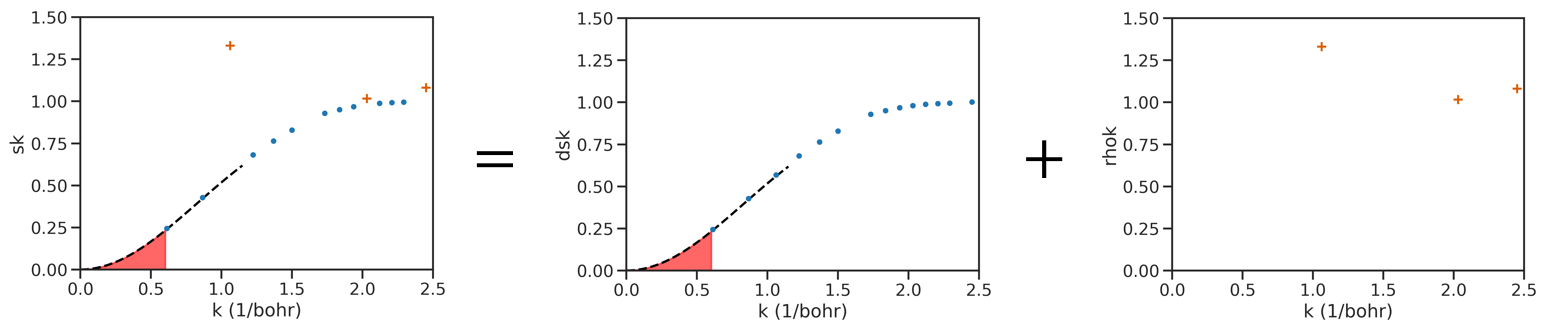
\includegraphics[width=\linewidth]{fsc-sk-dsk-rhok}
\caption{Fluctuating and static contributions from valence electrons in the conventional cell of bulk silicon.}
\label{fig:fsc-sk-dsk-rhok}
\end{figure}
As shown in Fig.~\ref{fig:fsc-sk-dsk-rhok}, the static part due to charge density $\rho_{\bs{k}}$ is non-zero only at reciprocal lattice of the primitive cell of the underlying crystal structure, whereas the fluctuating part varies smoothly from $0$ to $1$. Its value within the missing $\bs{k}=\bs{0}$ region (red area in Fig.~\ref{fig:fsc-sk-dsk-rhok}) can be used to correct the potential energy to leading order following eq.~(\ref{eq:fsc-dvn-missing}).
Changes in the charge density with system size is a higher-order effect and is small compared to the total potential energy~\cite{Clay2016}. However, as shown in Ref.~\cite{Yang2020-gap}, this static contribution becomes important when energy differences are taken, such as in the calculation of the fundamental gap.

Equation~(\ref{eq:wf-gaskell-rpa-sk}) still works well at $k\ll k_F$, but the short-range contribution $S_0(k)$ no longer comes from a simple determinant of plane waves. For insulators, dielectric screening suppresses long-range fluctuation and changes the leading-order behavior of $S(k)$ from eq.~(\ref{eq:wf-gaskell-rpa-sk-taylor}) to eq.~(7) in Ref.~\cite{Yang2020-gap}
\begin{align}
S(k) \approx \dfrac{k^2}{2\omega_p}(1-\epsilon_k^{-1})^{1/2},
\end{align}
so long as plasmons are the dominant excitation in the system.

\section{Correction to the kinetic energy}

\subsection{From momentum distribution}
The kinetic energy can be calculated as the second moment of the momentum distribution
\begin{align} \label{eq:fsc-tn-nk}
T_N \equiv T/N = \frac{1}{\rho}\int \dfrac{d^d\bs{k}}{(2\pi)^d} e(k) n_N(\bs{k}),
\end{align}
where the dispersion of non-relativistic particles
\begin{align}
e(k) = \dfrac{\hbar^2}{2m} k^2,
\end{align}
and $n_N(\bs{k})$ is the momentum distribution of these particles at the given system size $N$. It is crucial to distinguish the finite-size $n_N(\bs{k})$ from its thermodynamic limit $n_{\infty}(\bs{k})$, because it is a nonlocal quantity that converges slowly with system size~\cite{Holzmann2009}.
Similar to eq.~(\ref{eq:fsc-dvn}), the finite-size correction to the kinetic energy
\begin{align} \label{eq:fsc-dtn-nk}
\Delta T_N = \left[
\dfrac{1}{\rho}\int \dfrac{d^d\bs{k}}{(2\pi)^d} e(k)n_{\infty}(\bs{k})
\right] - \left[
\dfrac{1}{N}\sum\limits_{\bs{k}}
e(k)n_N(\bs{k})
\right].
\end{align}
The key difficulty in using eq.~(\ref{eq:fsc-dtn-nk}) is finding a reasonable approximation to $n_{\infty}(\bs{k})$. Some progress can be made by analyzing the Monte Carlo estimator for the Fourier transform of the momentum distribution, i.e. the off-diagonal one-particle density matrix~\cite{W.L.McMillan1965}
\begin{align} \label{eq:fsc-nr}
n(\bs{r}) = \left\langle \dfrac{\Psi(\bs{R}:\bs{r}_i\rightarrow\bs{r})}{\Psi(\bs{R})} \right\rangle_{\vert\Psi\vert^2},
\end{align}
where $\bs{R}$ denotes the positions of all $N$ particles, and the notation ``$:\bs{r}_i\rightarrow\bs{r}$'' means that particle $i$ is moved from $\bs{r}_i$ to $\bs{r}$.
As noted by W.R. Magro and D.M. Ceperley~\cite{Magro1994}, direct application of eq.~(\ref{eq:fsc-nr}) with periodic boundary condition can result in superfluous contributions, because all periodic images of particle $i$ are moved. The images will contribute to the ratio in eq.~(\ref{eq:fsc-nr}) if $\Psi$ has long-range components, e.g., eq.~(\ref{eq:fsc-rpa-wf}). Chiesa et al.~\cite{Chiesa2007} and Holzmann et al.~\cite{Holzmann2009} later used this observation to design a finite-size correction to the momentum distribution and the kinetic energy. To leading-order~\cite{Holzmann2009}
\begin{align} \label{eq:fsc-dnk-lo}
n_{\infty}(\bs{k}) - n_N(\bs{k}) \approx \int_{\frac{(2\pi)^d}{\Omega}}
\dfrac{d^d\bs{q}}{(2\pi)^d}
\left[
u_{\bs{q}}(1-S(\bs{q}))-\rho u(\bs{q})^2S(\bs{q})
\right]
\left(
n_N(\bs{k}+\bs{q})-n_N(\bs{k})
\right),
\end{align}
where $u_{\bs{q}}$ is the Jastrow pair potential in the wave function eq.~(\ref{eq:fsc-rpa-wf}).
As shown in Fig.~8 of Ref.~\cite{Yang2020-licp}, the leading-order correction to $n(\bs{k})$ works well for lithium. Further, Table~III in the Supplemental materials of Ref.~\cite{Yang2020-licp} shows that the corrected $n_N(\bs{k})$ can be used to accurately correct the finite-size error in the kinetic energy using eq.~(\ref{eq:fsc-dtn-nk}). To achieve this good result for a metal with a sharp Fermi surface such as lithium, it is crucial to densely sample momentum space while preserving the Fermi surface using grand-canonical twist averaging.

\subsection{From wave function}
Instead of using the relation between kinetic energy and the momentum distribution eq.~(\ref{eq:fsc-tn-nk}), one can directly analyze the QMC estimator for kinetic energy to find its finite-size correction. The VMC estimator for the kinetic energy of a Slater-Jastrow wave function $\Psi=De^{-U}$ is (from eq.~(14) of Ref.~\cite{Holzmann2016})
\begin{align} \label{eq:fsc-tn-vmc}
T_N^{VMC} = \frac{1}{N}\left\langle
-\sum\limits_{i=1}^N \dfrac{\hbar^2}{2m}\left[
\dfrac{\nabla_i^2D}{D} - (\bs{\nabla}_i U)^2
\right]
\right\rangle\equiv T_N^D + T_N^U.
\end{align}
The dominant finite-size correction in the determinant term is due to one-particle ``shell filling'' effects, whereas the dominant correction in the Jastrow term is due to long-range two-particle correlation. I will now discuss these two effects in turn.
\subsubsection{Single-particle ``shell filling'' effect}
If the orbitals in the determinant are from some effective one-particle theory such as HF or KS-DFT, then they are solutions of some effective one-particle potential $\veff$
\begin{align}
\left[
-\dfrac{\hbar^2\nabla^2}{2m} + \veff
\right] \phi_n(\bs{r}) = \epsilon_n\phi_n(\bs{r}).
\end{align}
Thus, one can work out the determinant contribution to the kinetic energy
\begin{align} \label{eq:fsc-tdn}
T^D_N \equiv -\dfrac{\hbar^2}{2m}\sum\limits_{i=1}^N \dfrac{\nabla_i^2D}{D} = \left[
\sum\limits_{n=1}^N\epsilon_n - \sum\limits_{i=1}^N \veff(\bs{r}_i)
\right],
\end{align}
by eq.~(19) in Ref.~\cite{Holzmann2016}. As the number of electrons is increased, the kinetic contribution eq.~(\ref{eq:fsc-tdn}) increases by the energies of the new orbitals being occupied. Consider the ideal Fermi gas in a 2D square box. As the number of same-spin particles increase from $N=2$ to $5$, the first shell of states in reciprocal space become filled. They all have the same single-particle energy, so the total kinetic energy increases linearly with $N$. However, when one adds a 6$^{\text{th}}$ particle, it increases the total energy by twice the amount as one in the first shell. As shown in Fig.~\ref{fig:fsc-lin-tabc}, this shell filling effect causes oscillation in the kinetic energy as a function of the number of particles, making size extrapolation difficult. This shell filling effect can be drastically reduced by adopting canonical twist averaged boundary conditions (TABC), where the number of particles is the same across all twists. Further, grand-canonical twist averaged boundary condition (GC-TABC), where the number of particles change to according to the exact Fermi surface, can exactly remove this single-particle finite-size effect. Finally, there is another ``pocket'' method which reduces the number of twists needed. Within a pocket in reciprocal space, the orbitals in the determinant smoothly acquire a phase as the twist is varied. Once these pockets are mapped out, one can perform one calculation per pocket and weigh it by the volume of the pocket to exactly remove the one-particle finite-size error~\cite{Holzmann2016}.

\begin{figure}[h]
\centering
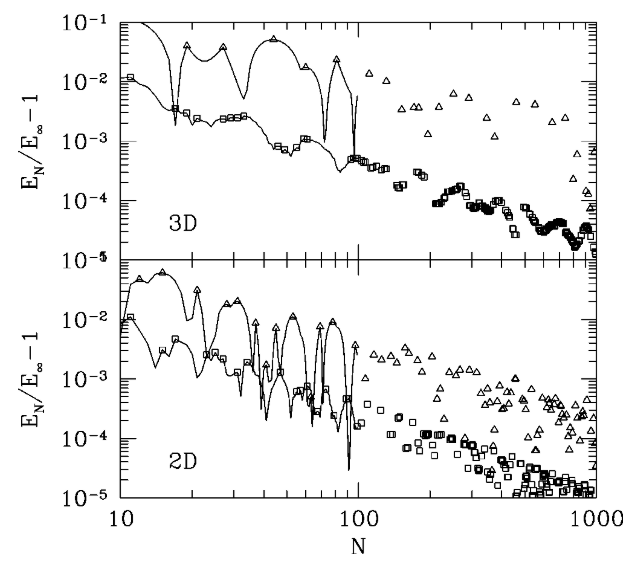
\includegraphics[width=0.6\linewidth]{lin-tabc}
\caption{Relative error of total energy vs. number of particles with PBC (up triangles) and TABC (squares) in 2D and 3D~\cite{Lin2001}}
\label{fig:fsc-lin-tabc}
\end{figure}

\subsubsection{Two-body size effect}
Using the RPA Jastrow pair potential from eq.~(\ref{eq:fsc-rpa-wf}), its contribution to eq.~(\ref{eq:fsc-tn-vmc}) becomes
\begin{align} \label{eq:fsc-tn-uk-sk}
T^U_N \equiv \dfrac{1}{N}\left\langle
\sum\limits_{i=1}^N \dfrac{\hbar^2}{2m} (\bs{\nabla}_iU)^2
\right\rangle
\approx \frac{1}{\Omega} \sum\limits_{\bs{k}\neq\bs{0}}
 \dfrac{\hbar^2}{2m} \rho u_{\bs{k}}u_{-\bs{k}}S(\bs{k}),
\end{align}
by eq.~(33) in Ref.~\cite{Holzmann2016}.
Recall the general relation between $S(\bs{k})$ and $u(\bs{k})$ eq.~(\ref{eq:uk-sk})
\begin{align}
2\rho u_{\bs{k}} \approx S^{-1}(\bs{k}) - S^{-1}_0(\bs{k}).
\end{align}
Since $S^{-1}(\bs{k})$ diverges faster than $S_0^{-1}(\bs{k})$ as $k\rightarrow0$, eventually $2\rho u_{\bs{k}} \approx S^{-1}(\bs{k})$. Thus, to leading-order eq.~(\ref{eq:fsc-tn-uk-sk}) becomes
\begin{align} \label{eq:fsc-tn-uk-ek}
T_N^U \approx \dfrac{1}{2\Omega} \sum\limits_{\bs{k}\neq\bs{0}}
e(k)u_{\bs{k}},
\end{align}
which should be compared with eq.~(\ref{eq:fsc-vn-vk}) for potential energy. Thus, the procedure to correct the two-body finite-size error in the kinetic energy is analogous to the potential correction scheme eq.~(\ref{eq:fsc-dvn})
\begin{align} \label{eq:fsc-dtn-uk}
\Delta T_N \equiv T_{\infty} - T_N = \left[
\int \dfrac{d^d\bs{k}}{(2\pi)^d} - \dfrac{1}{\Omega}\sum\limits_{\bs{k}}
\right] \frac{e(k)}{2} u(\bs{k}),
\end{align}
where $u(\bs{k})$ is an interpolation of the converged Jastrow pair potential, which can be approximated using the converged static structure factor in the long wavelength limit.

\subsubsection{Finite-temperature correction}
\textit{Based on notes from D. M. Ceperley}\\
At finite temperature and under the RPA, the long-range part of the action can be optimized to minimize the variance of the local energy, resulting in
\begin{align} \label{eq:fsc-finitet-uk}
2\rho u_k = Q(\bs{k}, \beta)^{-1}\tanh\left(
\dfrac{\beta}{2}\dfrac{e(k)}{Q(\bs{k}, \beta)}
\right) - S_0(\bs{k},\beta)^{-1},
\end{align}
where $\beta$ is inverse temperature, $e(k)=\lambda k^2$ is the dispersion of the particle, $\rho=N/\Omega$ is density, and $S_0(\bs{k}, \beta)$ is the non-interacting structure factors.
\begin{align}
Q(\bs{k}, \beta) \equiv \left(S_0(\bs{k}, \beta)^{-2}+\dfrac{2\rho v_{\bs{k}}}{e(k)}\right)^{-1/2}.
\end{align}
$Q(\bs{k}, \beta)$ reduces to Gaskell RPA $S(\bs{k})$ as $\beta\rightarrow\infty$. Since $\lim\limits_{x\rightarrow\infty}\tanh(x)=1$, eq.~(\ref{eq:fsc-finitet-uk}) becomes eq.~(\ref{eq:uk-sk}) in this limit. Assuming the relation between $S(\bs{k})$ and $u_{\bs{k}}$ eq.~(\ref{eq:uk-sk}) holds, the finite-temperature RPA structure factor is
\begin{align} \label{eq:fsc-finitet-sk}
S(\bs{k},\beta) = Q(\bs{k},\beta)/\tanh\left(
\dfrac{\beta}{2}\dfrac{e(k)}{Q(\bs{k}, \beta)}
\right).
\end{align}
Equations~(\ref{eq:fsc-finitet-uk}) and (\ref{eq:fsc-finitet-sk}) can be used to derived leading-order finite-size corrections to the kinetic and potential energies using eq.~(\ref{eq:fsc-dtn-uk}) and (\ref{eq:fsc-dvn}), respectively.

\begin{comment}
\section{Overview}
How does finite size error scale with system size?

What are typical methods used to deal with finite-size error?
1. extrapolation based on Fermi-liquid theory. For bosons?
2. rely on effective one-particle theory e.g. HF and DFT.
3. two-body finite-size correction

\section{Periodic boundary condition (PBC)}
There are two types of finite-size errors in simulations with periodic boundary condition. The first is the artificial correlation between periodic images.

% Fermi liquid

% Chiesa

% MPC

% KZK

\section{Thermodynamic limit}
The key quantity to consider in QMC is the local energy
\begin{align}
E_L = -\sum\limits_i \lambda_i \left[
\dfrac{\nabla_i^2D}{D} - (\nabla_iU)^2 - \nabla_iU\nabla_i(U_{FN}-U)
\right] + V.
\end{align}

\subsection{Shell-filling effect}
\subsection{Electronic structure factor $S(k)$}
\subsection{Jastrow pair function $U(k)$}
\subsection{Electronic momentum distribution $n(k)$}
\section{Grand-canonical twist-averaged boundary condition (GC-TABC)}
\end{comment}